\documentclass[11pt]{article}

\usepackage{fullpage}
\usepackage{hyperref}
\usepackage{graphicx}


\begin{document}

\title{Group 9 Project Report}
\author{Patrick Henderson\\
	\and
	Sukant Roy\\
	\and 
	Kapilan Manu Neethi Cholan\\
	\and 
	Jordan Bunke
}

\maketitle

\section{Emulator}

\section{Assembler}

\section{Extension}

\subsection{Background}

The chosen extension was to implement a stack into the emulator. For this, space needs to be defined for the stack in the memory component of the emulator along with operations to manipulate the stack (pushing and popping). The ARM instruction set includes Block Data Transfer instructions: \texttt{ldm} - to transfer multiple words of memory to registers and \texttt{stm} - to transfer the contents of multiple registers to memory. These can be used to perform popping to and pushing from the stack respectively.\\
\indent The implemented stack will conform to the properties of a descending stack in the sense that it will grow towards lower memory addresses. In other words, the data pushed most recently onto the stack will have a lower memory address than data that already existed on the stack.\\
\indent Furthermore, the \texttt{branch} instruction in the ARM instruction set has another option: \texttt{branch and link} which can be implemented to simulate the effect of function calls in the emulator. \\
\indent A stack can be used to implement the effect of function calls, preserving the contents of registers on the stack and storing the memory address of the instruction for which control should resume once a called subroutine has terminated execution. This feature is absent from the current implementation of the emulator implemented thus far. Furthermore, the \texttt{ldm} and \texttt{stm} instructions are very efficient for saving and restoring the contents of registers and moving large quantities of data in memory.

\subsection{Design}

\subsubsection{Stack}

Currently, the emulator has \texttt{64KB} of memory. Rather than extending this to accommodate for a stack, it was decided to allocate a portion of this memory to act as one. The chosen size of the stack is \texttt{8KB}; $2^{13} = 8192$  bytes and $\frac{1}{8}$ of the memory. 
A stack usually operates with a \texttt{base pointer} and a \texttt{stack pointer}, which are registers in some architectures, such as x84-64. In the ARM architecture, the stack pointer is Register 13 and there is no base pointer register.\footnote{\label{stackpointerfoot} \url{https://www.cs.virginia.edu/~skadron/cs433\_s09\_processors/arm11.pdf} Page 5} Alternatively, a constant can be used to define the base of the stack, so the bottom of the stack is defined as the last word of memory: \texttt{0x0000FFFC}, as demonstrated in Figure \ref{fig:memory}.

\begin{figure}[h!]
	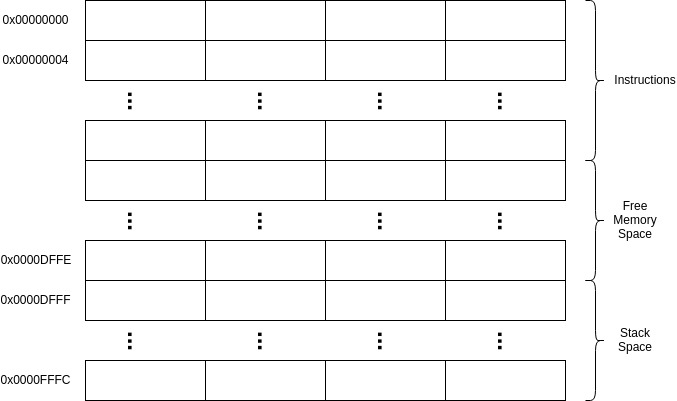
\includegraphics[width=\linewidth]{memory.jpg}
	\caption{Memory in the emulator.}
	\label{fig:memory}
\end{figure}

To detect stack overflow, after each instruction has executed in the emulator pipeline, a check will be performed with the value in the stack pointer register and the base of the stack to ensure that the difference of these two values does not exceed \texttt{8KB}.

\subsubsection{Block Data Transfer}

\subsection{Testing}

Given that the extension enhances the functionality of the emulator and assembler, the test suite used for these was able to be used for testing the extension. 

\section{Group Organisation}

\section{Reflections}

\subsection{Group Reflection}

\subsection{Individual Reflections}

\subsubsection{Patrick Henderson}

\subsubsection{Sukant Roy}

\subsubsection{Kapilan Manu Neethi Cholan}

\subsubsection{Jordan Bunke}

\end{document}
